%!TEX options = --shell-escape
% This is a magic comment that tells LatexTools to enable shell-escape
% If you're not using LatexTools to compile, you will need to enable shell escape on your editor

%%%%%%%%%%%%%%%%%%%%%%%%%%%%%%%%%%%%%%%%%%%%%%%%%%%%%%%%%%%%%%%%%%%%%%%%%%%%%%%%%
%
% <Name of your project here>
% 	by Charles Baynham
% 	30 May, 2018
%
% Based on template by Charles Baynham,
% modified from template by Ajeet Sandu
% https://www.overleaf.com/latex/templates/requirements-specification-layout/vbrqbjpzcmfy
%
%%%%%%%%%%%%%%%%%%%%%%%%%%%%%%%%%%%%%%%%%%%%%%%%%%%%%%%%%%%%%%%%%%%%%%%%%%%%%%%%%

\documentclass{article}

\usepackage{softwareRequirements}
\usepackage{standalone}
\usepackage{sphinx}

\begin{document}

\pagenumbering{roman}
\DeclareGraphicsExtensions{.pdf,.jpg,.png}

%% Table of contents
\tableofcontents

%% Version table insertion
%!TEX root = ../second_app_planning.tex

% This document defines the version history. Entries should include the git
% hash of the appropriate milestones

\section*{Revision History}
\addcontentsline{toc}{section}{Revision History}
\begin{versionhistory}
	\vhEntry{0.1 (\#58a9b4)}{2018/05/30}{CFAB}{Automatically generated quality documentation}
\end{versionhistory}

\clearpage
\pagestyle{long}

\pagenumbering{arabic}

% The content:
\graphicspath{{images/}}
\graphicspath{{./}}

\section{Introduction}\label{introduction}

This the quality document for the punpy software package.


The statement of work for this project defines the user requirements.

The functional requirements are included as a separate document in this folder as `Functional\_Requirements.docx'.

The software design is described in Section \ref{design}.

An automated test report is given in Section \ref{testreport}. This includes:
\begin{itemize}
\item A table detailing the environment that was used during testing.
\item A summary of the results, indicating how many tests passed and how long it took.
\item A table showing each of the tests that was run, how long they took, and what output was captured during testing.
\item A test coverage report, showing how many lines of the software were covered by the combined tests.
\end{itemize}

\clearpage
\section{Software design}\label{design}
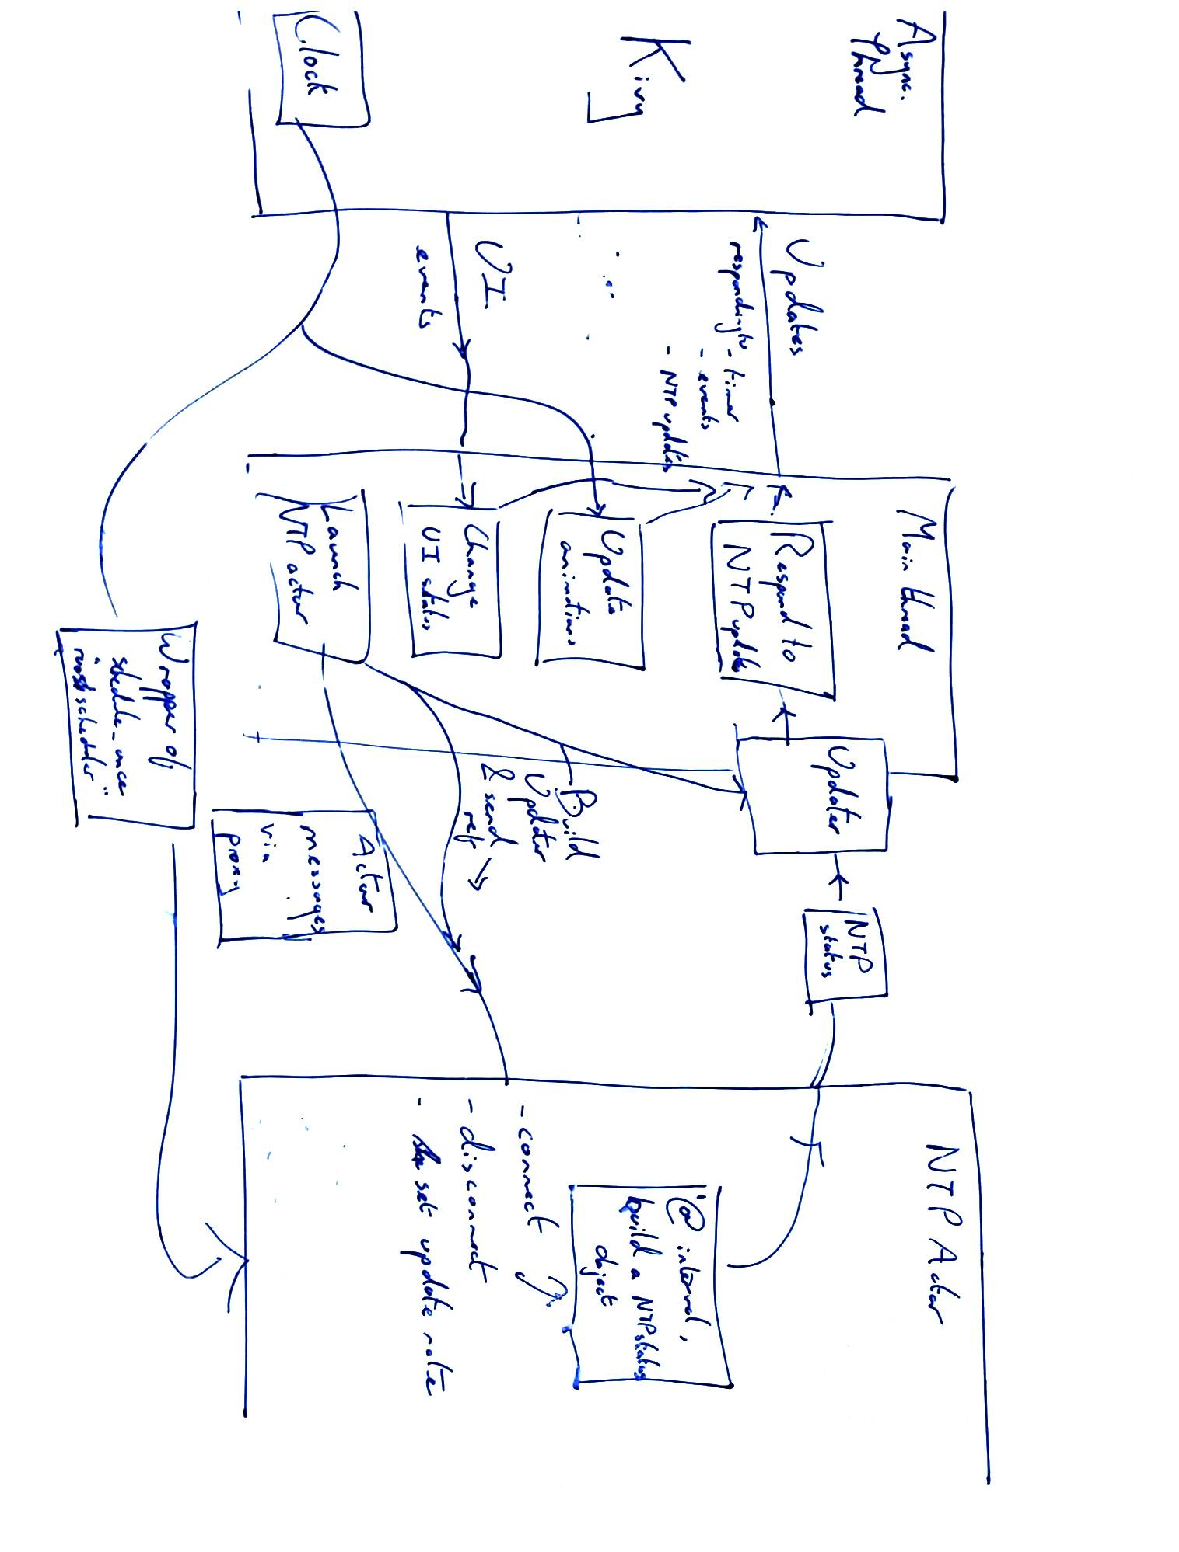
\includegraphics[width=\textwidth]{code_diagram.pdf}


\clearpage
\section{Test report}\label{testreport}

\input{test_report.tex}
\input{cov_report.tex}

\clearpage

\part*{User Manual}
\phantomsection
\addcontentsline{toc}{part}{User Manual}
\appendix
\def\maketitle{}
\def\tableofcontents{}
\input{./latex/punpy.tex}

\end{document}
